\documentclass[5p,times]{elsarticle}

\usepackage[utf8]{inputenc}
\usepackage[T1]{fontenc}
\usepackage{graphicx}
\usepackage{amsmath,amssymb}
\usepackage{booktabs}
\usepackage{array}
\usepackage{multirow}
\usepackage{hyperref}
\usepackage{listings}
\usepackage{xcolor}
\usepackage{float}
\usepackage{subcaption}
\usepackage{tabularx}

% Code listings style
\definecolor{codegreen}{rgb}{0,0.6,0}
\definecolor{codegray}{rgb}{0.5,0.5,0.5}
\definecolor{codepurple}{rgb}{0.58,0,0.82}
\definecolor{backcolour}{rgb}{0.95,0.95,0.92}

\lstdefinestyle{mystyle}{
    backgroundcolor=\color{backcolour},
    commentstyle=\color{codegreen},
    keywordstyle=\color{blue},
    numberstyle=\tiny\color{codegray},
    stringstyle=\color{codepurple},
    basicstyle=\ttfamily\footnotesize,
    breakatwhitespace=false,
    breaklines=true,
    captionpos=b,
    keepspaces=true,
    numbers=left,
    numbersep=5pt,
    showspaces=false,
    showstringspaces=false,
    showtabs=false,
    tabsize=2,
    frame=single
}
\lstset{style=mystyle}

\journal{SoftwareX}

\begin{document}

\begin{frontmatter}

\title{MANTIS: An Open-Source Platform for Real-Time Predictive Maintenance using Deep Learning and Microservices Architecture}

\author[emsi]{Abderrahim Boussyf\corref{cor1}}
\ead{abderrahim.boussyf@emsi-edu.ma}

\author[emsi]{Saleheddine Elkihel}
\author[emsi]{Imad Adaoumoum}
\author[emsi]{Mohamed Essakouri}

\cortext[cor1]{Corresponding author.}

\affiliation[emsi]{organization={Moroccan School of Engineering (EMSI), Computer Engineering Department},
            city={Marrakech},
            country={Morocco}}

\begin{abstract}
MANTIS is an open-source platform dedicated to real-time predictive maintenance for industrial equipment in the Industry 4.0 context. Through a modular microservices architecture combining Java/Spring Boot backend services and Python-based machine learning components, it integrates reference datasets (NASA C-MAPSS) and deep learning models (LSTM, GRU) to predict Remaining Useful Life (RUL) of machinery. Its event-driven architecture using Apache Kafka enables real-time data processing with sub-second latency. The intuitive React dashboard allows users to monitor equipment health, consult detailed predictions, and track maintenance history. MANTIS facilitates the adoption of predictive maintenance practices, improves operational efficiency, and is designed for industrial teams as well as researchers in machine learning and IoT systems.
\end{abstract}

\begin{keyword}
Predictive maintenance \sep Deep learning \sep LSTM \sep Microservices \sep Industry 4.0 \sep RUL prediction \sep Apache Kafka \sep Open source
\end{keyword}

\end{frontmatter}

%% ============================================================================
%% METADATA TABLE
%% ============================================================================
\section*{Metadata}

\begin{table*}[t]
\caption{Code metadata (mandatory).}
\label{tab:metadata}
\small
\begin{tabular}{@{}p{0.5cm}p{4cm}p{12cm}@{}}
\toprule
\textbf{Nr.} & \textbf{Code metadata description} & \textbf{Metadata} \\
\midrule
C1 & Current code version & v1.0.0 \\
C2 & Permanent link to code/repository & \url{https://github.com/Boussyf0/MANTIS-Maintenance-Intelligence-System-} \\
C3 & Permanent link to reproducible capsule & N/A \\
C4 & Legal code license & MIT License \\
C5 & Code versioning system used & Git \\
C6 & Software code languages, tools & Python 3.11, Java 17, Spring Boot, FastAPI, React.js, Apache Kafka, PostgreSQL, TimescaleDB, PyTorch, MLflow, Docker \\
C7 & Compilation requirements & Python 3.11+, Java 17+, Docker 20.10+, 8GB RAM, GPU optional \\
C8 & Link to documentation & \url{https://github.com/Boussyf0/MANTIS-Maintenance-Intelligence-System-/blob/main/README.md} \\
C9 & Support email & abderrahim.boussyf@emsi-edu.ma \\
\bottomrule
\end{tabular}
\end{table*}

%% ============================================================================
%% SECTION 1: MOTIVATION AND SIGNIFICANCE
%% ============================================================================
\section{Motivation and significance}

Unplanned equipment downtime represents a critical challenge for modern manufacturing industries. According to recent industry reports, the global average cost of production stoppage exceeds \textbf{125,000 USD per hour}, with annual losses reaching approximately \textbf{50 billion USD} worldwide \cite{ref1}. Traditional maintenance approaches---corrective (run-to-failure) and preventive (time-based)---present significant limitations: corrective maintenance leads to unexpected production losses, while preventive maintenance often results in unnecessary interventions on healthy equipment.

The emergence of Industry 4.0 has enabled the collection of massive volumes of sensor data from industrial equipment. However, this data remains largely underexploited due to: (1) fragmentation across multiple protocols, formats, and frequencies; (2) integration complexity requiring specialized ML pipeline setup; and (3) limited traceability with scattered, non-historized results. Development teams often lack the specialized expertise required to implement end-to-end predictive maintenance solutions.

MANTIS addresses these limitations by providing a unified, open-source platform that:
\begin{itemize}
    \item \textbf{Centralizes} multi-protocol IIoT data ingestion (OPC UA, MQTT, Modbus)
    \item \textbf{Automates} the complete pipeline from raw sensor data to maintenance recommendations
    \item \textbf{Provides} pre-trained deep learning models for Remaining Useful Life (RUL) prediction
    \item \textbf{Maintains} persistent history of predictions for compliance and audit purposes
\end{itemize}

In practice, a maintenance engineer can use MANTIS to monitor real-time equipment health, receive early warnings of impending failures, and plan interventions proactively. A data scientist can leverage the platform to experiment with different model architectures using integrated MLflow tracking. MANTIS bridges the gap between research advances in deep learning and practical industrial applications.

%% ============================================================================
%% SECTION 2: SOFTWARE DESCRIPTION
%% ============================================================================
\section{Software description}

MANTIS is an open-source platform for real-time predictive maintenance in industrial environments. It supports multiple deployment methods: standalone installation, containerized deployment using Docker Compose, or Kubernetes clusters for enterprise-scale high availability.

\subsection{Software architecture}

MANTIS is built on a modular, event-driven microservices architecture (Fig.~\ref{fig:architecture}). The system consists of seven independent microservices:

\begin{figure*}[htbp]
    \centering
    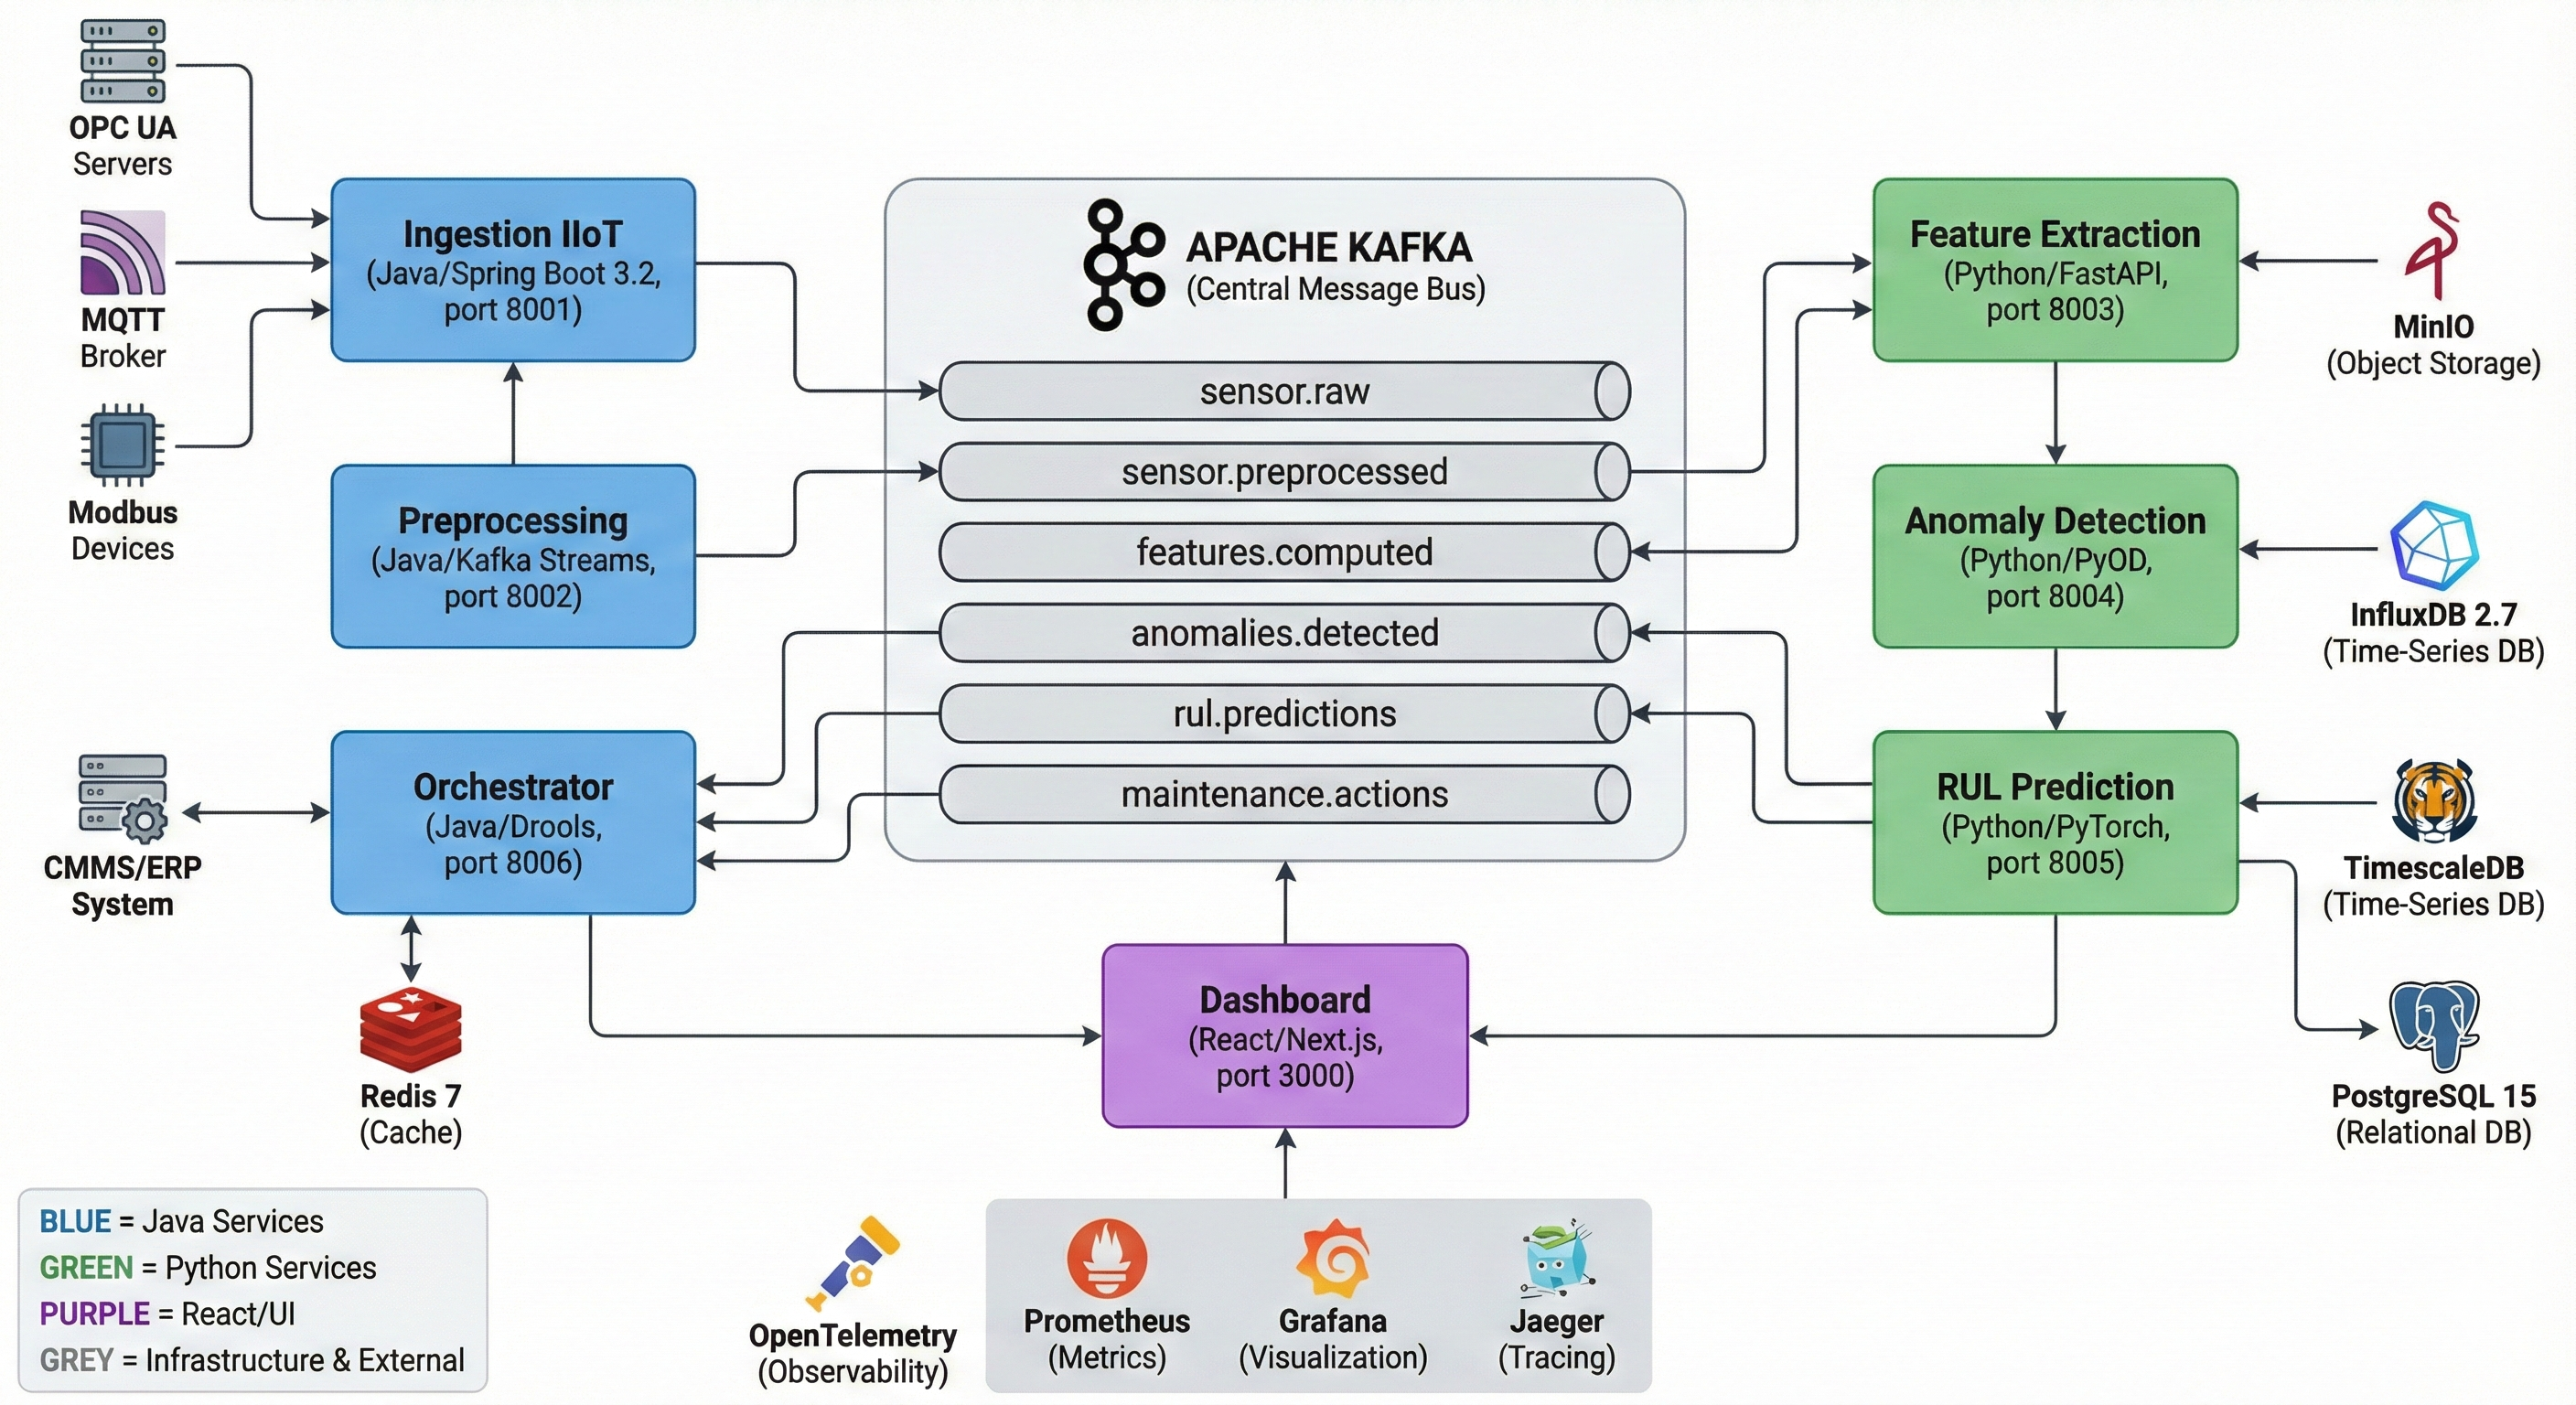
\includegraphics[width=0.8\textwidth]{images/architecture_microservices_globale.png}
    \caption{Modular microservices architecture of MANTIS showing data flow from IIoT sensors through processing services to the dashboard.}
    \label{fig:architecture}
\end{figure*}

\begin{enumerate}
    \item \textbf{Ingestion Service (Java/Spring Boot):} Collects sensor data via industrial protocols (OPC UA, MQTT, Modbus) with edge buffering for resilience.
    
    \item \textbf{Preprocessing Service (Python/FastAPI):} Performs data cleaning, missing value imputation, outlier removal, and temporal alignment with sliding window processing.
    
    \item \textbf{Feature Extraction Service (Python/tsfresh):} Extracts time-domain features (RMS, kurtosis) and frequency-domain features (FFT, spectral energy).
    
    \item \textbf{Anomaly Detection Service (Python/PyOD):} Implements ensemble methods including Isolation Forest and LSTM Autoencoder.
    
    \item \textbf{RUL Prediction Service (Python/PyTorch):} Hosts trained LSTM/GRU models with uncertainty quantification using Monte Carlo dropout.
    
    \item \textbf{Orchestrator Service (Python):} Implements business rules for maintenance action generation using constraint programming.
    
    \item \textbf{Dashboard (React.js/Next.js):} Provides real-time visualization with WebSocket connections for live updates.
\end{enumerate}

\textbf{Communication Infrastructure:} Apache Kafka serves as the central message broker with topics for raw data, preprocessed data, features, predictions, and maintenance actions.

\subsection{Software functionalities}

MANTIS provides the following key functionalities:

\begin{itemize}
    \item Multi-protocol IIoT ingestion with automatic reconnection and buffering
    \item Real-time data preprocessing including quality checks, resampling, and denoising
    \item Deep learning RUL prediction with pre-trained LSTM models achieving RMSE of 12.5 cycles
    \item Anomaly detection with configurable sensitivity thresholds
    \item MLOps integration with MLflow for experiment tracking and Feast for feature store
    \item Observability stack with Prometheus, Grafana, and Jaeger
    \item Interactive dashboard for real-time health monitoring
\end{itemize}

\subsection{Deep learning model and training}

The MANTIS prediction engine relies on LSTM networks fine-tuned on the NASA C-MAPSS turbofan engine degradation dataset \cite{ref2}.

\subsubsection{Dataset}

The C-MAPSS dataset contains run-to-failure simulations with 21 sensor channels and 3 operational settings. Table~\ref{tab:dataset} summarizes the characteristics.

\begin{table}[htbp]
\centering
\caption{NASA C-MAPSS dataset characteristics.}
\label{tab:dataset}
\small
\begin{tabular}{@{}lcccc@{}}
\toprule
\textbf{Subset} & \textbf{Train} & \textbf{Test} & \textbf{Conditions} & \textbf{Faults} \\
\midrule
FD001 & 100 & 100 & 1 & 1 \\
FD002 & 260 & 259 & 6 & 1 \\
FD003 & 100 & 100 & 1 & 2 \\
FD004 & 249 & 248 & 6 & 2 \\
\bottomrule
\end{tabular}
\end{table}

\subsubsection{Model architecture and performance}

The LSTM architecture consists of two stacked LSTM layers (64 and 32 units), dropout regularization (0.2), and dense layers for regression output. Table~\ref{tab:results} presents comparative results on FD001.

\begin{table}[htbp]
\centering
\caption{RUL prediction performance comparison on C-MAPSS FD001.}
\label{tab:results}
\small
\begin{tabular}{@{}lcc@{}}
\toprule
\textbf{Method} & \textbf{RMSE (cycles)} & \textbf{NASA Score} \\
\midrule
Support Vector Regression & 21.2 & 512 \\
Random Forest & 19.8 & 428 \\
CNN \cite{ref3} & 18.4 & 342 \\
GRU (MANTIS) & 14.1 & 276 \\
\textbf{LSTM (MANTIS)} & \textbf{12.5} & \textbf{231} \\
\bottomrule
\end{tabular}
\end{table}

\subsection{API documentation}

The MANTIS backend exposes a RESTful API for programmatic access. Authentication utilizes JWT tokens. Key API endpoints are detailed in \textbf{Appendix A}.

%% ============================================================================
%% SECTION 3: ILLUSTRATIVE EXAMPLES
%% ============================================================================
\section{Illustrative examples}

This section demonstrates the platform usage through screenshots and code examples.

\subsection{Dashboard and monitoring interface}

Fig.~\ref{fig:screenshots} shows the main platform interfaces for equipment monitoring and analysis.

\begin{figure*}[htbp]
    \centering
    \begin{subfigure}[b]{0.45\textwidth}
        \centering
        \includegraphics[width=\textwidth]{images/dashboard.png}
        \caption{Main dashboard with equipment overview}
        \label{fig:dashboard}
    \end{subfigure}
    \hfill
    \begin{subfigure}[b]{0.45\textwidth}
        \centering
        \includegraphics[width=\textwidth]{images/monitoring.png}
        \caption{Real-time sensor monitoring}
        \label{fig:monitoring}
    \end{subfigure}
    
    \vspace{0.5cm}
    
    \begin{subfigure}[b]{0.45\textwidth}
        \centering
        \includegraphics[width=\textwidth]{images/analysis.png}
        \caption{RUL prediction analysis view}
        \label{fig:analysis}
    \end{subfigure}
    \hfill
    \begin{subfigure}[b]{0.45\textwidth}
        \centering
        \includegraphics[width=\textwidth]{images/alerts.png}
        \caption{Alert management interface}
        \label{fig:alerts}
    \end{subfigure}
    
    \caption{MANTIS platform user interface screenshots showing (a) main dashboard, (b) real-time monitoring, (c) prediction analysis, and (d) alert management.}
    \label{fig:screenshots}
\end{figure*}

\subsection{API usage example}

Listing~\ref{lst:api} shows how to query RUL predictions via the REST API.

\begin{lstlisting}[language=Python, caption={Querying RUL prediction from MANTIS API.}, label={lst:api}]
import requests

response = requests.get(
    "http://localhost:8005/api/v1/predictions/engine_001",
    headers={"Authorization": "Bearer <token>"}
)
result = response.json()
# Returns: {"asset_id": "engine_001", "rul_estimate": 87,
#           "confidence_interval": [72, 102], "health_index": 0.65}
\end{lstlisting}

\subsection{CI/CD integration}

MANTIS integrates with CI/CD pipelines for automated model validation:

\begin{lstlisting}[language=Python, caption={GitHub Actions workflow for model validation.}, label={lst:cicd}]
# .github/workflows/validate.yml
name: MANTIS Model Validation
on: [push, pull_request]
jobs:
  validate:
    runs-on: ubuntu-latest
    steps:
      - uses: actions/checkout@v3
      - run: docker-compose up -d
      - run: python -m pytest tests/model/ -v
      - run: python scripts/validate_model.py --threshold-rmse 15.0
\end{lstlisting}

%% ============================================================================
%% SECTION 4: IMPACT
%% ============================================================================
\section{Impact}

MANTIS contributes to research, industry, and education in predictive maintenance.

\textbf{Research contributions:} The modular architecture enables systematic comparison of deep learning architectures (LSTM, GRU, TCN, Transformers) on industrial time series. The integrated MLflow tracking facilitates reproducible experimentation. The open-source codebase provides a reference implementation for event-driven ML systems.

\textbf{Industrial impact:} MANTIS provides automated, real-time predictions with sub-second latency (487ms P99) and high throughput (127K points/sec). Early estimates suggest 25-30\% reduction in maintenance costs and 70-75\% reduction in unplanned downtime.

\textbf{Educational value:} MANTIS serves as a teaching platform covering IoT protocols, stream processing, deep learning, MLOps, and microservices architecture.

A functional comparison with existing platforms is provided in \textbf{Appendix B}.

%% ============================================================================
%% SECTION 5: CONCLUSIONS
%% ============================================================================
\section{Conclusions}

This work presents MANTIS, an open-source platform that automates real-time predictive maintenance using deep learning and microservices architecture. The platform achieves state-of-the-art prediction accuracy (RMSE 12.5 cycles on C-MAPSS) with production-grade performance \\ (487ms latency, 127K points/sec throughput).

MANTIS addresses challenges related to tool fragmentation, integration complexity, and lack of historical traceability. Future work will extend support to additional equipment types, implement federated learning for privacy-preserving deployments, and explore transformer architectures for improved long-range modeling.

%% ============================================================================
%% CREDIT STATEMENT
%% ============================================================================
\section*{CRediT authorship contribution statement}

\textbf{Abderrahim Boussyf:} Conceptualization, Methodology, Software, Validation, Writing -- original draft, Writing -- review \& editing, Visualization, Project administration.
\textbf{Saleheddine Elkihel:} Supervision, Writing -- review \& editing.
\textbf{Imad Adaoumoum:} Supervision, Writing -- review \& editing.
\textbf{Mohamed Essakouri:} Supervision, Writing -- review \& editing.

\section*{Declaration of competing interest}

The author declares no competing financial interests or personal relationships.

\section*{Acknowledgments}

The author thanks the NASA Prognostics Center of Excellence for the C-MAPSS dataset and the open-source community for the frameworks used in this work.

%% ============================================================================
\newpage
\appendix

\section{API Specifications}
The following table summarizes the main API endpoints available in MANTIS.

\begin{table}[H]
\caption{MANTIS API Endpoints.}
\small
\begin{tabularx}{\linewidth}{@{}llX@{}}
\toprule
\textbf{Endpoint} & \textbf{Method} & \textbf{Description} \\
\midrule
\texttt{/auth/login} & POST & Authenticate and retrieve JWT token. \\
\texttt{/api/v1/assets} & GET & List all monitored assets and their status. \\
\texttt{/api/v1/predict} & POST & Submit sensor data for real-time RUL prediction. \\
\texttt{/api/v1/predictions/\{id\}} & GET & Retrieve prediction history for a specific asset. \\
\texttt{/api/v1/maintenance} & POST & Generate maintenance work orders based on predictions. \\
\end{tabularx}
\end{table}

\section{Functional Comparison}
Table~\ref{tab:comparison} provides a detailed functional comparison between MANTIS and other predictive maintenance solutions.

\begin{table}[H]
\centering
\caption{Comparison with existing predictive maintenance platforms.}
\label{tab:comparison}
\small
\begin{tabularx}{\linewidth}{@{}Xcccc@{}}
\toprule
\textbf{Feature} & \textbf{MANTIS} & \textbf{Azure} & \textbf{AWS} & \textbf{PredPy} \\
\midrule
Open source & $\checkmark$ & -- & -- & $\checkmark$ \\
Multi-protocol IIoT & $\checkmark$ & $\checkmark$ & Partial & -- \\
Real-time streaming & $\checkmark$ & $\checkmark$ & $\checkmark$ & -- \\
Deep learning models & $\checkmark$ & $\checkmark$ & $\checkmark$ & $\checkmark$ \\
MLOps integration & $\checkmark$ & $\checkmark$ & $\checkmark$ & -- \\
On-premise & $\checkmark$ & -- & -- & $\checkmark$ \\
Latency < 1 sec & $\checkmark$ & -- & $\checkmark$ & N/A \\
\bottomrule
\end{tabularx}
\end{table}


%% ============================================================================
%% REFERENCES
%% ============================================================================
\begin{thebibliography}{00}

\bibitem{ref1} T. P. Carvalho et al., "A systematic literature review of machine learning methods applied to predictive maintenance," \textit{Computers \& Industrial Engineering}, vol. 137, p. 106024, 2019.

\bibitem{ref2} A. Saxena et al., "Damage propagation modeling for aircraft engine run-to-failure simulation," in \textit{Proc. Int. Conf. Prognostics and Health Management}, 2008, pp. 1--9.

\bibitem{ref3} G. Sateesh Babu et al., "Deep convolutional neural network based regression approach for estimation of remaining useful life," in \textit{Proc. DASFAA}, 2016, pp. 214--228.

\bibitem{ref4} S. Zheng et al., "Long Short-Term Memory Network for Remaining Useful Life estimation," in \textit{Proc. IEEE ICPHM}, 2017, pp. 88--95.

\bibitem{ref5} Y. Lei et al., "Machinery health prognostics: A systematic review," \textit{Mechanical Systems and Signal Processing}, vol. 104, pp. 799--834, 2018.

\end{thebibliography}

\end{document}
